\documentclass[tikz,border=2pt]{standalone}
\usetikzlibrary{arrows.meta,positioning,shapes.geometric,calc}
\begin{document}
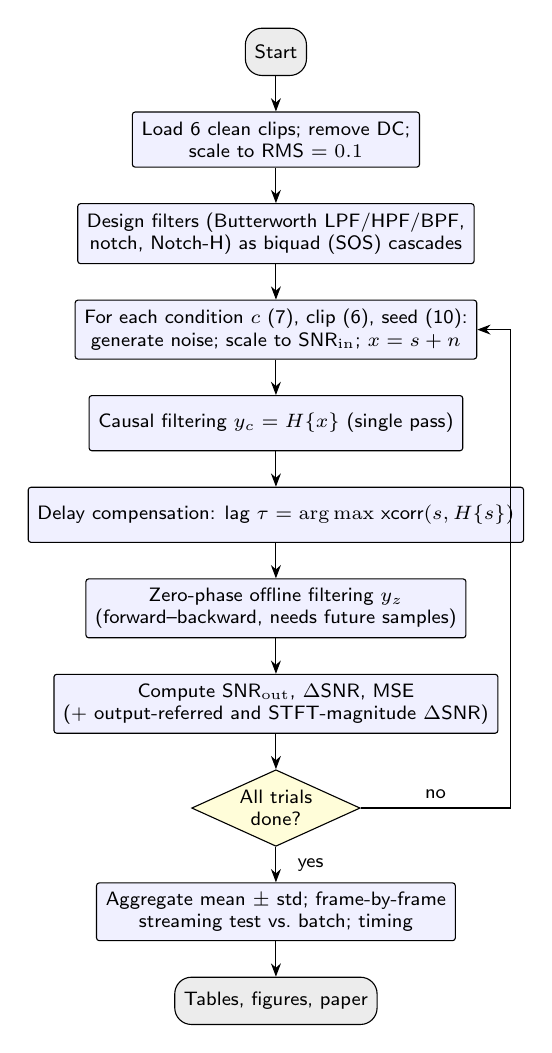
\begin{tikzpicture}[font=\sffamily\scriptsize,>=Stealth,node distance=0.45cm and 0.5cm,
  p/.style={draw,rounded corners=1pt,minimum height=0.7cm,minimum width=3.6cm,align=center,fill=blue!6},
  d/.style={draw,diamond,aspect=2.2,inner sep=1pt,align=center,fill=yellow!15},
  t/.style={draw,rounded corners=6pt,minimum height=0.6cm,align=center,fill=gray!15}]
\node[t] (s) {Start};
\node[p,below=of s] (a) {Load 6 clean clips; remove DC;\\scale to RMS $=0.1$};
\node[p,below=of a] (b) {Design filters (Butterworth LPF/HPF/BPF,\\notch, Notch-H) as biquad (SOS) cascades};
\node[p,below=of b] (c) {For each condition $c$ (7), clip (6), seed (10):\\generate noise; scale to SNR$_\mathrm{in}$; $x=s+n$};
\node[p,below=of c] (e) {Causal filtering $y_c=H\{x\}$ (single pass)};
\node[p,below=of e] (f) {Delay compensation: lag $\tau=\arg\max$ xcorr$(s,H\{s\})$};
\node[p,below=of f] (g) {Zero-phase offline filtering $y_z$\\(forward--backward, needs future samples)};
\node[p,below=of g] (h) {Compute SNR$_\mathrm{out}$, $\Delta$SNR, MSE\\(+ output-referred and STFT-magnitude $\Delta$SNR)};
\node[d,below=of h] (i) {All trials\\done?};
\node[p,below=of i] (j) {Aggregate mean $\pm$ std; frame-by-frame\\streaming test vs.\ batch; timing};
\node[t,below=of j] (k) {Tables, figures, paper};
\foreach \u/\v in {s/a,a/b,b/c,c/e,e/f,f/g,g/h,h/i,i/j,j/k} \draw[->] (\u) -- (\v);
\draw[->] (i.east) -- ++(1.9,0) node[above,pos=0.5]{no} |- (c.east);
\node[right=0.05cm of $(i.south)!0.5!(j.north)$,xshift=0.1cm] {yes};
\end{tikzpicture}
\end{document}
